152. \begin{figure}[ht!]
\center{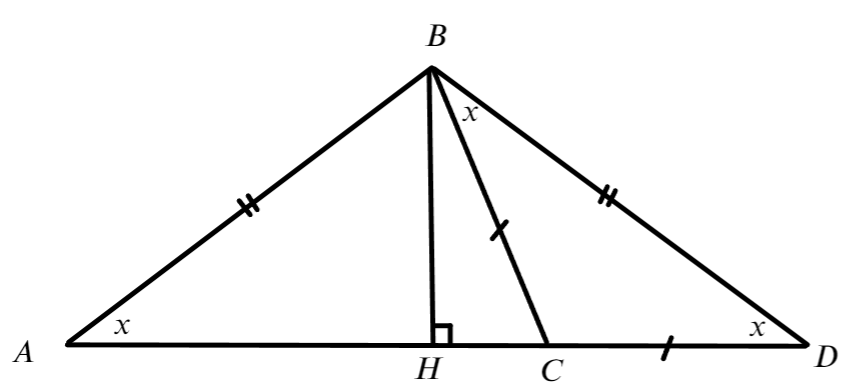
\includegraphics[scale=0.35]{g7-152.png}}
\end{figure}\\
Отметим на продолжении стороны $AC$ точку $D$ так, чтобы $DC=BC.$ Тогда $DH=DC+CH=BC+CH=AH,$ а значит в треугольнике $ABD$ высота $BH$ совпала с медианой, поэтому он является равнобедренным. Отметив равные углы в равнобедренных треугольниках $BCD$ и $ABD$ и написав сумму углов треугольника $ABD,$ получим $3x+84^\circ=180^\circ,\ x=32^\circ.$ Значит, $\angle BAC=32^\circ.$\\
